\documentclass[UTF8,a4paper,11pt]{ctexart}
\usepackage[margin=22mm]{geometry}
\usepackage{amsmath,amssymb,bm}
\usepackage{booktabs,tabularx,array}
\usepackage{graphicx}
\usepackage{xcolor}
\usepackage{hyperref}
\usepackage{caption}
\usepackage{float}
\usepackage{setspace}
\setstretch{1.15}
\hypersetup{colorlinks=true,linkcolor=black,citecolor=black,urlcolor=blue}
\captionsetup{font=small,labelfont=bf}
\title{\vspace{-8mm}Reference-Relative Generative Information Design\\[4pt]
\large 实验定稿：主结果、机制分析、真实数据与校准附录}
\author{RR-GID 实验定稿 \quad 2026-09-13}
\date{}

\begin{document}
\maketitle
\vspace{-6mm}
\noindent\textit{相对 2026-08-20 八页草稿的实验落地说明。}理论章节仍见原稿第 1--5 节。本节报告已完成并 fail-closed 审计通过的正文实验。原稿中的 VAEAC、exact oracle、\(J\) 消融、Gas 50 replication、以及 C2ST/RMSE 主表，按 2026-09-02 重规划不再作为正文主结果。

\section{实际执行协议}

正文只回答三个问题：固定预算下 RR-GID 是否降低 target 全分布误差；优势是否来自非线性条件信息；冻结生成器能否跨 campaign 复用。真实数据只验证 drift 下是否仍成立。

\paragraph{统一指标。}
合成数据主指标为
\[
R_{\mathrm{risk}}=\frac{B\cdot\mathrm{KL}(Q_{\beta^\star}\Vert Q_{\widehat\beta})}{C^\star},\qquad
C^\star=\tfrac12\Phi_{\beta^\star}(p^\star),
\]
越低越好，\(R_{\mathrm{risk}}=1\) 为 oracle 一阶效率参考。Gas 主指标为 family-projection loss \(D_{\widehat A}(\widehat\beta,\beta^\dagger)\)。

\paragraph{后端，而非 exact oracle。}
全部 bulk 使用 validated fixed/cached QMC：score order 14，information order 12。order-14 cached 与 fixed 的最大绝对差为 \(6.0\times10^{-9}\)。正文不得写成 exact oracle。

\paragraph{生成器。}
合成数据使用冻结 GMM+warp 条件 oracle。Gas 原稿拟用 VAEAC，但 VAEAC 未过 RISK-2/3。工程等价替换为冻结经验 \(k\)NN（与 RISK-2 参考算子相同，Spearman \(=1\)、top-10 overlap \(=10/10\)）。C2ST 对 \texttt{ref\_val} 约 \(0.48\)--\(0.53\)。正文必须写明：Gas 生成器是冻结经验 \(k\)NN，不是 VAEAC。

\paragraph{格子。}
E1：200 paired replications，\(B\in\{2000,4000,8000,16000,32000\}\)，\(J=2\)。
E2：15 replications，\(B=8000\)，\(\alpha\in\{0,0.5,1.0,1.5\}\)，\(J=4\)。
E3：5 sequence \(\times\) 50 campaign，\(T\in\{1,5,20,50\}\)，RR-GID vs Discriminative Score OED。
E5：R1/R2 各 20 replications。
E4：最小校准，不进主图。

\section{Figure 1：合成主结果}

\begin{figure}[H]
\centering
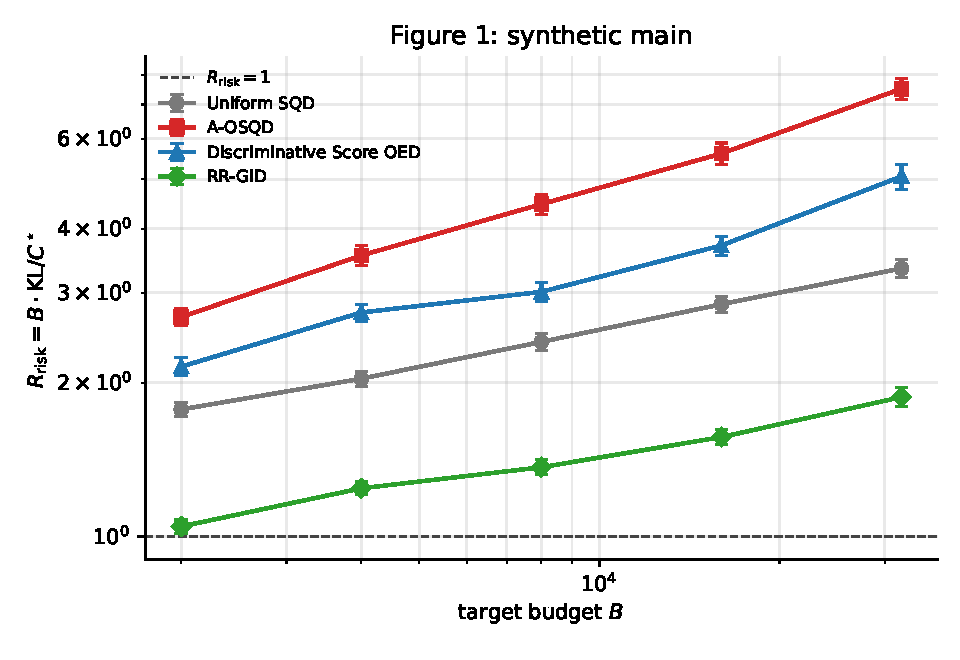
\includegraphics[width=0.82\textwidth]{figures/fig1_synthetic_main.pdf}
\caption{合成主实验（E1）。横轴 target budget \(B\)，纵轴 \(R_{\mathrm{risk}}\)。200 个配对 replication。RR-GID 全程低于 Uniform；A-OSQD 与 Discriminative Score OED 在该格子上不优于 Uniform。}
\end{figure}

最大预算 \(B=32000\)（Table~1a）：RR-GID 均值 \(1.88\)，Uniform \(3.35\)，相对改善 \(43.9\%\)，配对 bootstrap 95\% CI 为 \([1.23,1.72]\)（对 paired difference，不含 0）。A-OSQD \(7.51\)、Disc \(5.06\)，均差于 Uniform。不要把自适应政策写成全面优于均匀设计。

\section{Figure 2：非线性与生成器复用}

\begin{figure}[H]
\centering
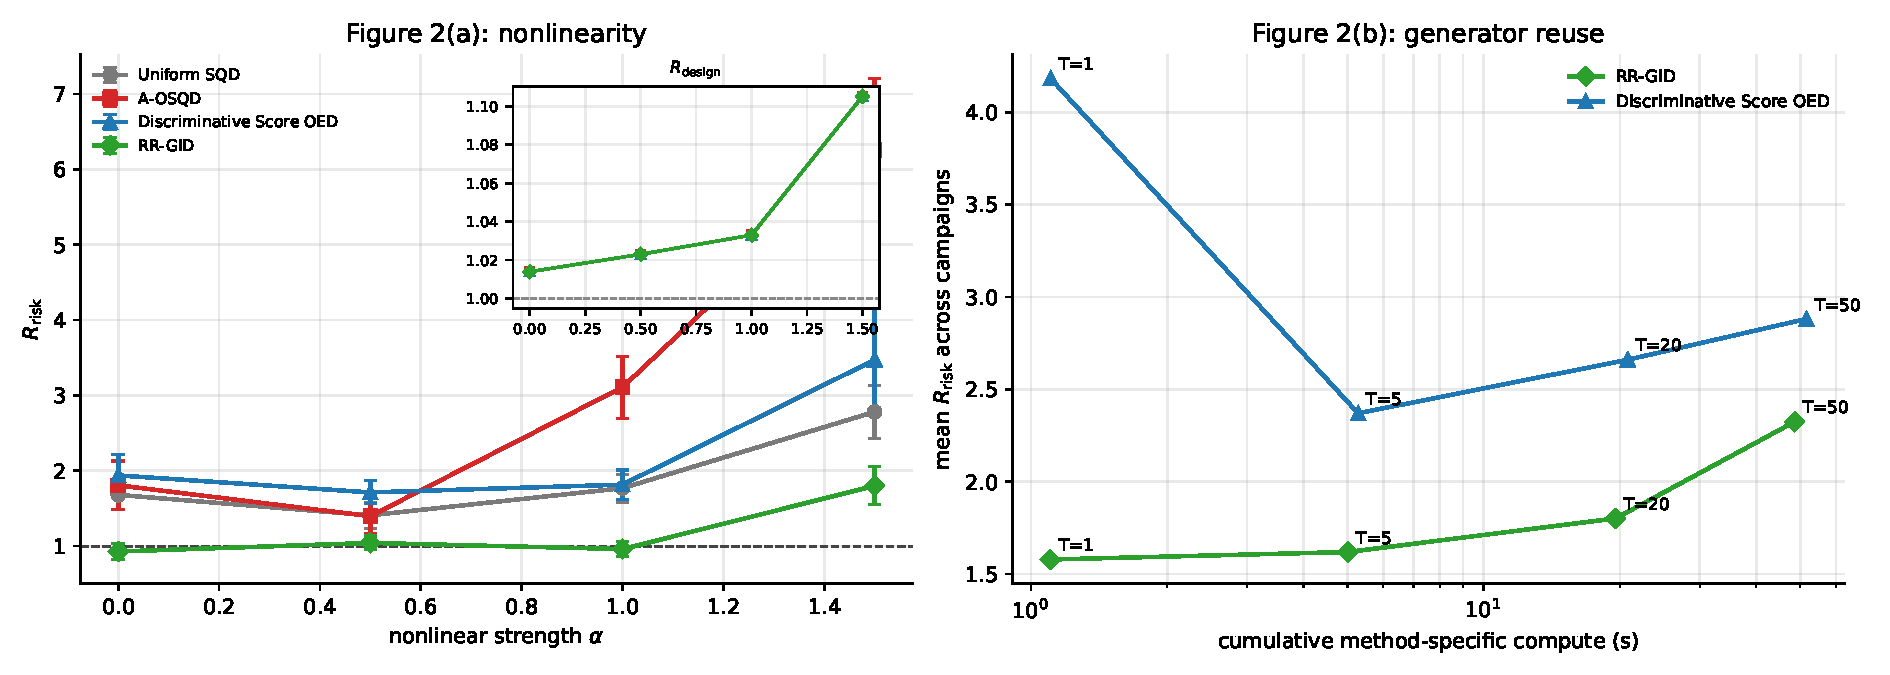
\includegraphics[width=\textwidth]{figures/fig2_mechanisms.pdf}
\caption{左：非线性强度 \(\alpha\)（E2，15 rep）。右：冻结生成器复用（E3，5 sequence）。}
\end{figure}

E2 中 RR-GID 在 \(\alpha\le 1\) 贴着一阶参考（\(0.93/1.04/0.96\)）；\(\alpha=1.5\) 升至 \(1.80\)，仍低于 Uniform \(2.78\) 与 Disc \(3.47\)。A-OSQD 在强非线性崩溃（\(6.26\)）。这支持机制 A：优势来自非线性条件信息，而不是协方差信息。

E3 在 \(T=50\)：RR-GID \(1.06\) vs Disc \(1.21\)。Disc 在 \(T=1\) 与 \(T=20\) 方差很大（\(T=20\) 均值 \(4.69\)，SE \(2.66\)）。仅 5 条 sequence，正文只报告趋势，不报告精确倍数。

\section{Figure 3：Gas Sensor Drift}

\begin{figure}[H]
\centering
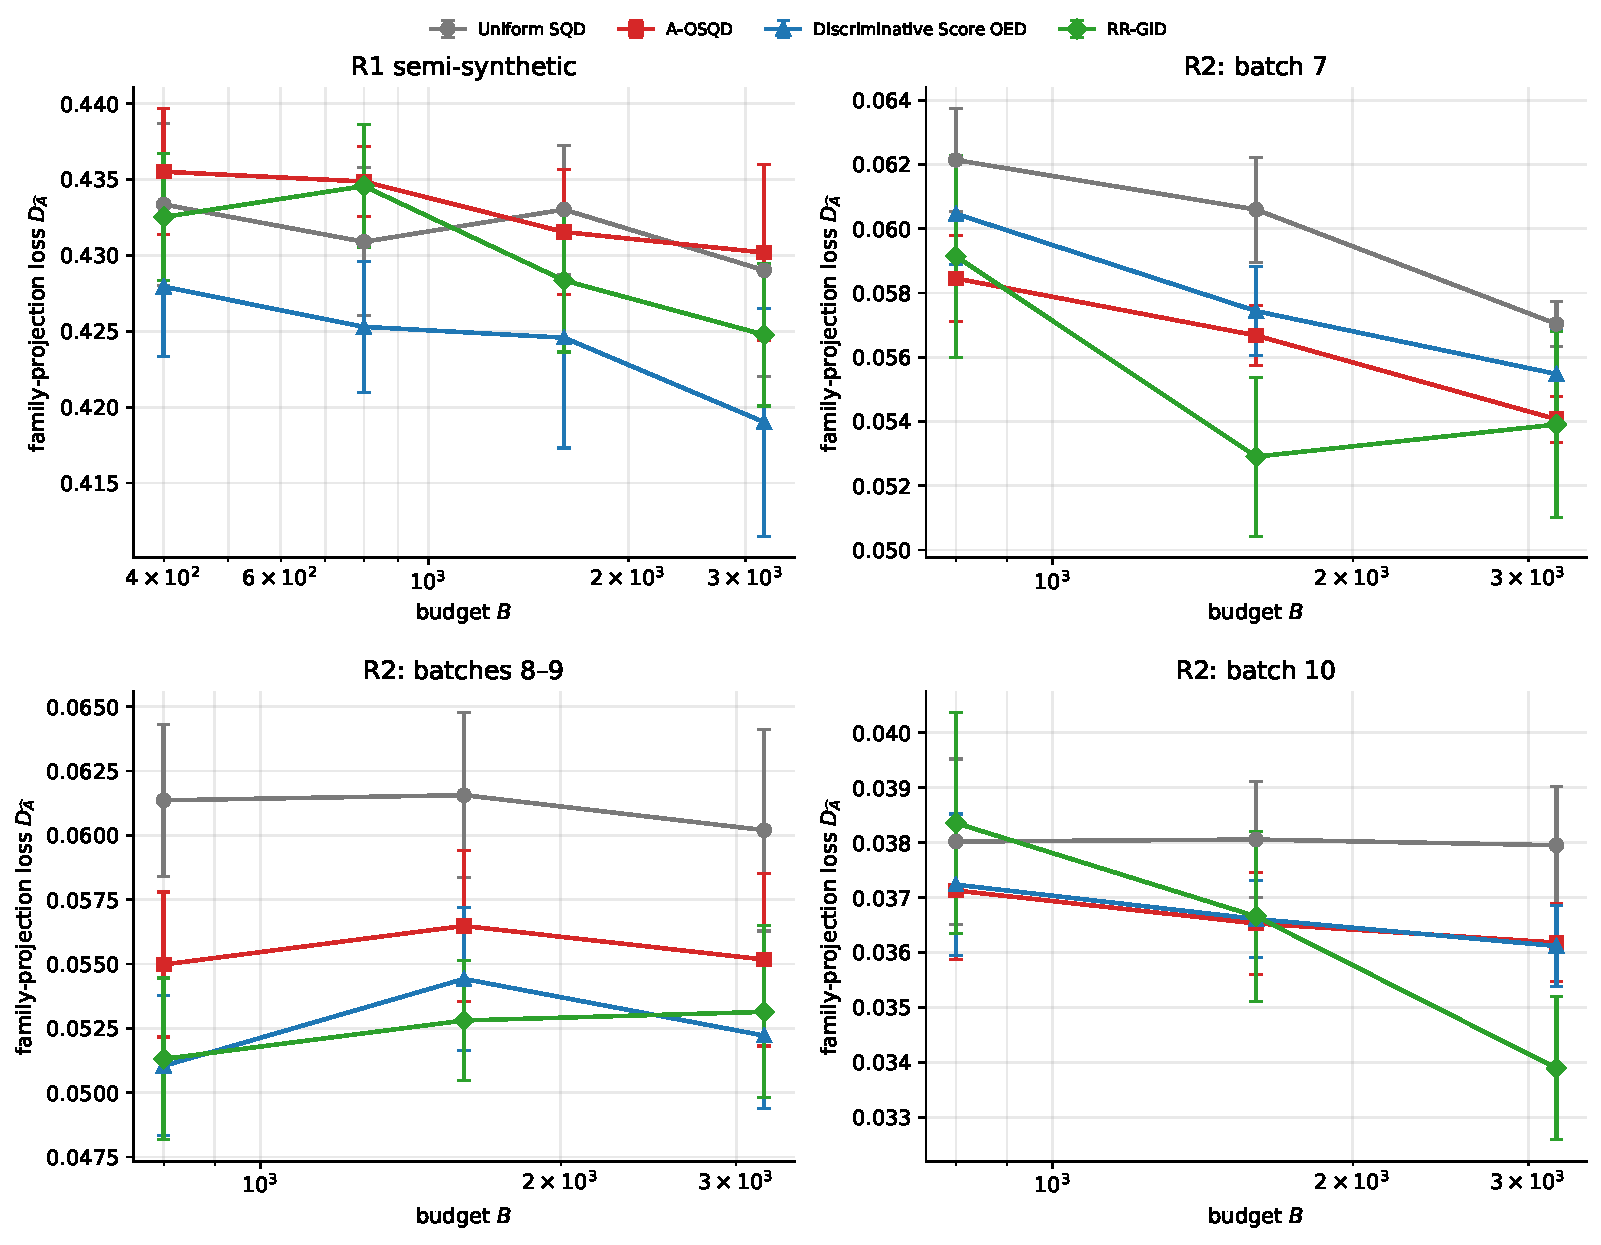
\includegraphics[width=\textwidth]{figures/fig3_gas.pdf}
\caption{上左：R1 well-specified 半合成。其余三格：R2 自然 drift（batch 7、8--9、10）。纵轴 family-projection loss。}
\end{figure}

R1 四方法 CI 重叠。\(B=3200\)：Disc \(0.419\)、RR-GID \(0.425\)、Uniform \(0.429\)。well-specified 设定下没有可报告的赢家。

R2 是主故事。相对 Uniform，RR-GID 在多数 campaign\(\times\)大预算更低，例如 batch~7、\(B=1600\)：\(0.053\) vs \(0.061\)；batch~10、\(B=3200\)：\(0.034\) vs \(0.038\)。Discriminative Score OED 仍是强基线，不写成碾压。

\section{Table 1：最大预算汇总}

只报告最大 \(B\) 的 primary loss、相对 Uniform 的配对改善、以及 95\% 配对 bootstrap CI。设计比 \(R_{\mathrm{design}}\) 在合成格子上由共享 target draw 决定，方法间相同，不作为区分证据。

\begin{table}[H]
\centering\small
\caption{Table 1a. 合成主实验，\(B=32000\)，\(n=200\)。loss 为 \(R_{\mathrm{risk}}\)。CI 为相对 Uniform 的配对差。}
\begin{tabular}{lrrrr}
\toprule
方法 & loss & \(\Delta\) vs Uniform & CI low & CI high \\
\midrule
Uniform SQD & 3.346 & 0.0\% & 0.000 & 0.000 \\
A-OSQD & 7.514 & \(-124.5\)\% & \(-4.809\) & \(-3.560\) \\
Discriminative Score OED & 5.062 & \(-51.3\)\% & \(-2.261\) & \(-1.217\) \\
RR-GID & 1.876 & \(+43.9\)\% & 1.229 & 1.717 \\
\bottomrule
\end{tabular}
\end{table}

\begin{table}[H]
\centering\small
\caption{Table 1b. Gas R1 半合成，\(B=3200\)，\(n=20\)。loss 为 projection loss。配对 CI 含 0，与 Figure~3 上左一致。}
\begin{tabular}{lrrrr}
\toprule
方法 & loss & \(\Delta\) vs Uniform & CI low & CI high \\
\midrule
Uniform SQD & 0.4290 & 0.0\% & 0.000 & 0.000 \\
A-OSQD & 0.4302 & \(-0.3\)\% & \(-0.009\) & 0.006 \\
Discriminative Score OED & 0.4190 & \(+2.3\)\% & \(-0.004\) & 0.027 \\
RR-GID & 0.4248 & \(+1.0\)\% & \(-0.010\) & 0.015 \\
\bottomrule
\end{tabular}
\end{table}

\begin{table}[H]
\centering\small
\caption{Table 1c. Gas R2 自然 drift，\(B=3200\)，每格 \(n=20\)。}
\begin{tabular}{llrr}
\toprule
campaign & 方法 & loss & vs Uniform \\
\midrule
batch 7 & Uniform SQD & 0.0570 & --- \\
batch 7 & A-OSQD & 0.0541 & 更低 \\
batch 7 & Discriminative Score OED & 0.0555 & 更低 \\
batch 7 & RR-GID & 0.0539 & 最低 \\
batches 8--9 & Uniform SQD & 0.0602 & --- \\
batches 8--9 & A-OSQD & 0.0552 & 更低 \\
batches 8--9 & Discriminative Score OED & 0.0522 & 最低 \\
batches 8--9 & RR-GID & 0.0531 & 更低 \\
batch 10 & Uniform SQD & 0.0380 & --- \\
batch 10 & A-OSQD & 0.0362 & 更低 \\
batch 10 & Discriminative Score OED & 0.0361 & 更低 \\
batch 10 & RR-GID & 0.0339 & 最低 \\
\bottomrule
\end{tabular}
\end{table}

\section{诚实限制}

\begin{itemize}
\item 合成主结果用 validated fixed-QMC，不是 exact oracle。
\item Gas 生成器是冻结经验 \(k\)NN。RISK-2 Spearman \(=1\) 是因为候选算子与参考算子相同，不是对 VAEAC 的外推验证。
\item E3 只有 5 条 sequence，Disc 的 CI 很宽。
\item R1 well-specified 下四方法不可分；真实数据故事在 natural drift。
\item 原稿 Fig.~4（C2ST / information fidelity 主图）与 \(J\in\{0,1,2\}\) 消融已从正文移除，校准只放附录。
\end{itemize}

\clearpage
\appendix
\section{E4：最小 oracle calibration}

Query 级（200 query，frozen order 12）：median relative error \(9.5\times10^{-4}\)，95th percentile \(2.2\times10^{-3}\)，max abs coordinate \(2.2\times10^{-3}\)，通过。

Information 级（20 panels \(\times\) 5 \(\beta\)，order 12）：allocation-weighted \(\|M_{\mathrm{gold}}^{-1/2}(\widehat M-M_{\mathrm{gold}})M_{\mathrm{gold}}^{-1/2}\|_{\mathrm{op}}\) 均值 \(0.0014\)、最大 \(0.0020\)，门限 \(0.05\)，通过。

End-to-end（\(B=8000\)，10 paired replications，fast order 14 vs gold adaptive 18）：mean \(|R_{\mathrm{fast}}-R_{\mathrm{gold}}|=0.038\le 0.15\)，且小于配对 SE \(0.017\)，通过（L2-e2e）。

RISK-2/3（经验 \(k\)NN）：information fidelity 与 C2ST-vs-\texttt{ref\_val} 通过。C2ST vs drifted target 接近 1，不作为开门条件。

\end{document}
